\chapter{Adaptive Filtering}

The previous chapter on wireless channel modeling established %
the wireless channel as a type of FIR filter. The aim of the %
receiver is to undo the effects of the channel filter. %
Figure \ref{fig:CommSysModel}. shows the communications %
system model as described in \cite{Sklar01}, for this section %
we'll draw our attention to the section of the model beginning %
at pulse modulation and ending at detection. 

\begin{figure}[h!]
	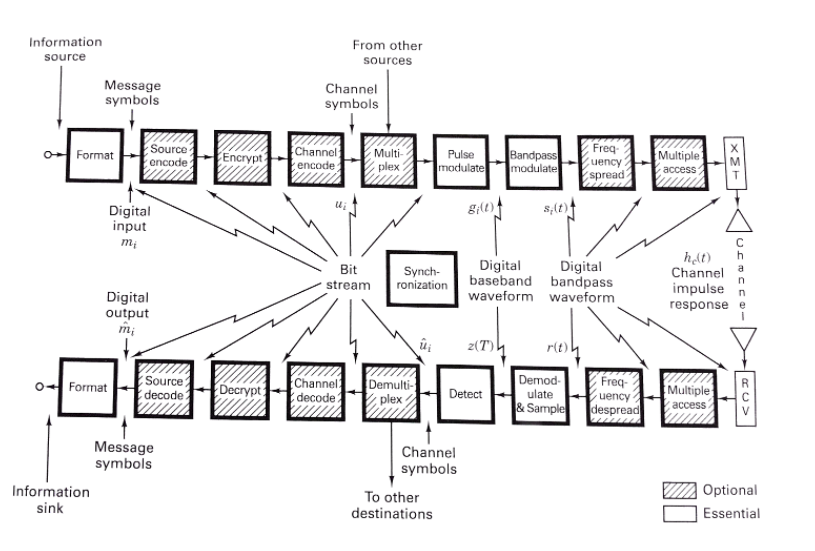
\includegraphics[width=\linewidth]{./Figures/Adaptive%
		Filters/CommunicationsSystemModel.png}
	\caption{Communications System Model \cite{Sklar01}}
	\label{fig:CommSysModel}
\end{figure}

The wireless system transfer function can be defined as:

\begin{align}
	H(f) = H_{t}(f)H_{c}(f)H_{r}(f)
\end{align}

where $H_{t}$ is the transfer function of the transmit filter, 
defined in the pulse modulate block, %
$H_{c}(f)$ is the transfer function of the channel, and $H_{r}%
(f)$ is the transfer function of the receive filter, defined in %
the demodulate and sample block. It's clear from this %
expression that the received baseband symbols at the %
detect block will be distorted by the channel filter $H_{c}%
(f)$, the goal of equalisation is to define an equalisation %
transfer function $H_{e}(f)$ that removes the effect of %
the channel filter. Such that the new system transfer %
function looks like this:

\begin{align}
	H(f) = H_{t}(f)H_{c}(f)H_{r}(f)H_{e}(f)
\end{align}

where

\begin{align}
	H_{c}(f)H_{e}(f) = 1
\end{align}



%TODO: insert diagram of the channel filter followed by
% an equalising filter

%TODO: provide a mathematical description of this equalisation
% effect

Throughout this entire chapter my development of adaptive filters %
will quite closely follow \cite{Hay02}. I'll start by %
developing the zero-forcing solution and the minimum mean square %
error solution also known as the Wiener solution. I'll then develop %
the stochastic gradient and the least mean square solution. A brief %
development of the recursive least square will be covered here as %
well.

\section{A Static Filter and The Wiener Solution}
% Need to introduce this section
\subsection{A Simple Filter the Zero-Forcing Solution}
\label{subsec:ZeroForcing}
Previously in chapter \ref{chap:OFDM} on OFDM, a key insight to %
the advantage of using the DFT was that the circular convolution %
in combination with the convolution theorem provided the nice %
property that the distortion introduced by the FIR channel filter %
introduced in chapter \ref{chap:ChannelModeling} can be represented %
as element wise multiplication in the frequency domain (see equation %
\ref{eq:DFTConvolutionTheorem}). It's clear that equation %
\ref{eq:ZeroForcing} does in fact represent a filtering operation %
in the frequency domain. This simple filter is commonly known as %
the zero forcing filter and is defined as the reciprocal of the %
frequency response of the channel filter $\frac{1}{H(f)}$. %
It's most easily found when a known set of symbols $X[i]$ have %
been transmitted such that
\begin{align}
	H\left[i\right] = \frac{Y\left[i\right]}{X\left[i\right]}
\end{align}
In a noiseless and time invariant environment this is the optimal %
solution to the equalisation problem. However a more accurate %
model for the received samples $y[nT]$ is
\begin{align}
	y[nT]=h[nT]\circledast x[nT]%
	+ v
\end{align}
where $h[nT]$ represents the channel filter of length %
$\mu$ at time $nT$ and $x[nT]$ are the inputs to %
$h[nT]$, $v$ represents the additive white gaussian %
noise (AWGN). Taking the DFT of both sides gives %
\begin{align}
	Y[i] = H[i]X[i] + V[i]%
	,\quad \text{ for } i = 0,1,\cdots,N-1
	\label{eq:AWGNModel}
\end{align}
Where $N$ is the length of the DFT. It's clear from %
equation \ref{eq:AWGNModel} that dividing through %
by $X[i]$ gives a noisy estimate of the channel %
frequency response
\begin{align}
	\frac{Y[i]}{X[i]} = H[i] + \frac{V[i]}{X[i]}, %
	\text{ for } i = 0,1,\cdots,N-1
\end{align}
equalising using this expression will lead to estimates %
of $X$
\begin{align}
	\hat{X}[i] =& \frac{H[i]X[i]+V[i]}{H[i]+V[i]/X[i]} \\
	=& \frac{H[i]X[i]}{H[i]+V[i]/X[i]} + \frac{V[i]}{H[i]
	+ V[i]/X[i]} \\
	=& \frac{H[i]}{H[i]+V[i]/X[i]}X[i] + 
	\frac{V[i]X[i]}{H[i]X[i]+V[i]}\\
	=& \frac{H[i]}{H[i]+V[i]/X[i]}X[i] + 
	\frac{V[i]X[i]}{Y[i]}
	\label{eq:NoiseAmplification}
\end{align}
Should $X[i]/Y[i]$ in equation \ref{eq:NoiseAmplification} %
be greater than $1$ then the noise in the received estimate %
$\hat{X}[i]$ will be amplified reducing SNR and increasing the bit %
error rate (BER).

\subsection{The Wiener Solution}
A solution to the noise amplification problem seen in %
section \ref{subsec:ZeroForcing} is to find the optimal %
solution taking noise into consideration. It's clear that %
this problem can be framed as an optimisation problem %
and so a measure of performance or cost function must %
first be defined to optimise. A natural choice for cost function %
is that of the mean square value of the estimation error. This %
is because the mean square error criterion results in a %
second order dependence for the cost function on the %
unknown coefficients in the impulse response of %
the filter. This leads to the cost function having a distinct %
minimum that uniquely defines the optimum %
statistical design of the filter \cite{Hay02}.
\subsubsection{The Wiener-Hopf Equations}
To develop this optimum solution first we revisit equation %
\ref{eq:BasebandChannelFIR} which describes the wireless channel %
as an FIR filter and for consistency with \cite{Hay02} and %
with my later development on my system model redefine it as
\begin{align}
	u(n) = \sum_{i}\tilde{h}(\tau)\tilde{s}(t-\tau)
	\label{eq:ChannelOut}
\end{align}
where $u(n)$ are now the series of inputs to an optimally %
designed filter with form shown in equation \ref{eq:FilterOut}. %
For the purposes of this chapter %
we will assume that the channel is time-invariant and set %
$\tilde{h}(\tau;t)$ to $\tilde{h}(\tau)$.
\begin{align}
	y(n) = \sum_{k=0}^{N-1}w_{k}^{*}u(n-k), n - 0,1,2,\cdots,N-1
	\label{eq:FilterOut}
\end{align}
where $u(n-k)$ are the discrete samples being received %
after having been distorted by the wireless channel, %
$w_{k}^{*}$ are the %
filter coefficients and the asterisk $^*$ represents %
complex conjugation. The estimation error will be defined as 
\begin{align}
	e(n) = d(n) - y(n)
	\label{eq:EstimationError}
\end{align}
where $d(n)$ is the desired output of the filter %
hence the %
mean square error criterion will be defined as
\begin{align}
	J =& E\left[e(n)e^{*}(n)\right]
	\label{eq:MeanSquareError}\\
	=& E\left[\lvert e(n) \rvert^{2}\right]
\end{align}
where $E\left[\cdot\right]$ denotes the expectation %
operator. With these definitions in mind the aim is now %
to minimise $J$. To do this the complex derivative of $J$ with %
respect to the filter coefficients $w_{k}^{*}$ needs %
to be found. First we'll define
\begin{align}
	w_{k}^{*} = a_{k} + jb_{k}
\end{align}
and 
\begin{align}
	\nabla_{k} = \frac{\partial}{\partial a_{k}} + j 
	\frac{\partial}{\partial b_{k}}
\end{align}
where $\nabla_{k}$ is the complex derivative %
operator with respect to $w_{k}^{*}$. From %
equations \ref{eq:FilterOut}, \ref{eq:EstimationError} %
and \ref{eq:MeanSquareError} %
\begin{align}
	\nabla_{k}J =& E\left[ \frac{\partial e(n)}
	{\partial a_{k}} e^{*}(n) + \frac{\partial
	e^{*}(n)}{\partial a_{k}}e(n) + \frac{
	\partial e(n)}{\partial b_{k}}je^{*}(n) 
	+ \frac{\partial e^{*}(n)}{\partial b_{
	k}}je(n)\right] \label{eq:DerivativeJ}
\end{align}
When evaluated 
\begin{align}
	\nabla_{k}J = -2E\left[u(n-k)e^{*}(n)\right]
	\label{eq:CostDerivative}
\end{align}
Since the mean square error criterion is quadratic %
the optimum solution can be found at its stationary %
point by setting
\begin{align}
	\nabla_{k}J =& 0,\quad\text{ for } k=0,1,2,\cdots,N-1
\end{align}
which implies that
\begin{align}
	E\left[u(n-k)e^{*}(n)\right] = 0,\quad\text{ for } k = 0,1,2,\cdots,N-1
	\label{eq:OptimalityCondition}
\end{align}
substituting equation \ref{eq:EstimationError} into %
\ref{eq:OptimalityCondition} gives
\begin{align}
	E\left[u(n-k)\left(d^{*}(n) - \sum_{m=0}^{N-1}w_{o_{m}}u
	^{*}(n-m)\right)\right]=0,\quad\text{ for }k=0,1,\cdots,N-1
\end{align}
where $w_{o_{m}}$ is the $m\text{th}$ coefficient of %
the impulse response of the optimum filter. Expanding and %
rearranging
\begin{align}
	&E\left[u(n-k)d^{*}(n) - u(n-k)\sum_{m=0}^{N-1}w
	_{o_{m}}u^{*}(n-m)\right] = 0\\
	\implies &E\left[u(n-k)d^{*}(n)\right] - E\left[u(n-k)\sum
	_{m=0}^{N-1}w_{o_{m}}u^{*}(n-m)\right] = 0\\
	\implies &E\left[u(n-k)d^{*}(n)\right] - \sum_{m=0}^{N-1}
	w_{o_{m}}E\left[u(n-k)u^{*}(n-m)\right] = 0\\
	\implies &E\left[u(n-k)d^{*}(n)\right] = 
	\sum_{m=0}^{N-1}w_{o_{m}}E\left[u(n-k)u^{*}(
	n-m)\right],\quad\text{for }k=0,1,\cdots,N-1
	\label{eq:ExpandedOptimalityCondition}
\end{align}
The expectation on the right side of equation %
\ref{eq:ExpandedOptimalityCondition} is the %
\emph{autocorrelation function} of the filter input %
for a lag of $m-k$ and can be expressed as
\begin{align}
	r(m-k) = E\left[u(n-k)u^{*}(n-m)\right]
	\label{eq:WienerAutocorrelation}
\end{align}
The expectation on the left side of equation %
\ref{eq:ExpandedOptimalityCondition} is the %
\emph{cross correlation} between the filter %
input and the desired response for a lag %
of $-k$ and can be expressed as
\begin{align}
	p(-k) = E\left[u(n-k)d^{*}(n)\right]
	\label{eq:WienerCrossCorrelation}
\end{align}
Substituting equations \ref{eq:WienerAutocorrelation} %
and \ref{eq:WienerCrossCorrelation} into %
\ref{eq:ExpandedOptimalityCondition} %
we get
\begin{align}
	\sum_{m=0}^{N-1}w_{o_{m}}r(m-k)=p(-k),\quad
	\text{for }k=0,1,\cdots,N-1
	\label{eq:WienerHopf}
\end{align}
The system of equations in \ref{eq:WienerHopf} %
define the optimal filter coefficients for the %
equaliser and are named the \emph{Wiener-%
Hopf equations}.
\subsubsection{Solution to the Wiener-Hopf Equations}
Matrix representations of the system of equations in %
\ref{eq:WienerHopf} will let us easily solve for %
the optimum filter coefficients $w_{o_{m}}$. %
Let $\bold{R}$ denote the $N$-by-$N$ correlation %
matrix of the vector of inputs to the optimal filter %
$\bold{u}(n) = [u(n),u(n-1),\cdots,u(n-(N-1))]^T$.
\begin{align}
	\bold{R} = E\left[\bold{u}(n)\bold{u}^{H}(n)\right]
\end{align}
where $^{T}$ denotes the transpose operation and %
$^{H}$ denotes the Hermitian or the complex conjugate %
tranpose operation. Similarly let $\bold{p}$ be the %
$N$-by-$1$ cross correlation vector between %
the inputs and the desired output. 
\begin{align}
	\bold{p} = E\left[\bold{u}(n)d^{*}(n)\right]
\end{align}
Equation \ref{eq:WienerHopf} may now be rewritten %
as
\begin{align}
	\bold{R}\bold{w_{o}} = \bold{p}
	\label{eq:WienerHopfMatrix}
\end{align}
where $\bold{w_{o}}$ denotes the $N$-by-$1$ optimal %
filter coefficient vector $[w_{o_{0}},w_{o_{1}},%
\cdots,w_{o_{N-1}}]^T$. To solve for $\bold{w_{o}}$ %
we simply premultiply both sides of equation %
\ref{eq:WienerHopfMatrix} by $\bold{R}^{-1}$ giving
\begin{align}
	\bold{w_{o}} = \bold{R}^{-1}\bold{p}
	\label{eq:WienerHopfSolution}
\end{align}
\section{Gradient Descent and the Least Mean Square}
The expectations in equations \ref{eq:WienerAutocorrelation} %
and \ref{eq:WienerCrossCorrelation} are usually not %
available to find $\bold{w}_{o}$. This motivates the %
need to develop an alternative way to estimate the %
optimal solution. One approach to finding this estimate %
is to find the solution using an iterative method using %
local information. I'll first develop the method of %
gradient descent as an iterative optimisation method %
which will naturally lead into an the Least Mean Square %
algorithm to estimate the optimal solution.
\subsection{Gradient Descent}
When considering the cost function $J(\cdot)$, %
the optimal solution can be defined as
\begin{align}
	J(\bold{w}_{o}) \leq J(\bold{w})\quad
	\text{for all }\bold{w}
\end{align}
The gradient descent method aims to iteratively %
solve for $J(\bold{w_{o}})$ by developing an %
algorithm with the following invariant
\begin{align}
	J(\bold{w}(n+1)) < J(\bold{w}(n))
\end{align}
starting with an arbitrary initial guess $\bold{w}(0)$. %
The method of steepest descent is a method which aims %
to achieve this by taking steps in the direction of %
of the optimal solution at each iteration. This can %
be done by finding the local direction of steepest %
descent defined as the negative of the gradient vector %
\begin{align}
	\bold{g} = \nabla J(\bold{w})
\end{align}
The algorithm is formally described by
\begin{align}
	\bold{w}(n+1) = \bold{w}(n) - \frac{1}{2}
	\mu\bold{g}(n)
	\label{eq:GradientDescent}
\end{align}
From equations \ref{eq:CostDerivative} and %
\ref{eq:WienerHopfMatrix} $\nabla J$ is
\begin{align}
	\nabla J(\bold{w}(n)) = 
	-2\bold{p} + 2\bold{R}\bold{w}(n)
	\label{eq:CostGradient}
\end{align}
substituting equation \ref{eq:CostGradient} into %
equation \ref{eq:GradientDescent}
\begin{align}
	\bold{w}(n+1) = \bold{w}(n) - \mu(
	\bold{R}\bold{w}(n) - \bold{p})
	\label{eq:WienerGradientDescent}
\end{align}
There are some problems around stability that %
need to be considered when using gradient descent. %
However as long as $\mu$ is chosen carefully this %
algorithm will converge to the optimal solution \cite{Hay02}.
\subsection{Least Mean Square}
The gradient descent method doesn't solve the problem of %
the expectations in equations \ref{eq:WienerAutocorrelation} %
and \ref{eq:WienerCrossCorrelation}. The simplest solution %
to this problem may instead be to use an instantaneous %
estimate of the autocorrelation
\begin{align}
	\hat{\bold{R}} = \bold{u}(n)\bold{u}^{H}(n)
	\label{eq:WienerAutocorrelationEstimate}
\end{align}
and an instantaneous estimate of the cross correlation
\begin{align}
	\hat{\bold{p}} = \bold{u}(n)d^{*}(n)
	\label{eq:WienerCrossCorrelationEstimate}
\end{align}
substituting equations \ref{eq:WienerAutocorrelationEstimate} %
and \ref{eq:WienerCrossCorrelationEstimate} into %
\ref{eq:WienerGradientDescent}
\begin{align}
	\hat{\bold{w}}(n+1) =&~\hat{\bold{w}}(n)-\mu(
	\hat{\bold{R}}\hat{\bold{w}}(n) - \hat{
	\bold{p}})\\
	=&~\hat{\bold{w}}(n) - \mu(\bold{u}(n)
	\bold{u}^{H}(n)\hat{\bold{w}}(n) - 
	\bold{u}(n)d^{*}(n))\\
	=&~\hat{\bold{w}}(n) - \mu\bold{u}(n)(
	\bold{u}^{H}(n)\hat{\bold{w}}(n) - d^{*}
	(n))
	\label{eq:LMSUpdate}
\end{align}
The new estimate of $\hat{\bold{w}}$ lead %
to a new filter output and error estimate %
using the estimate of $\bold{w_{o}}$ 
\begin{align}
	y(n) =&~\hat{\bold{w}}^{H}(n)\bold{u}(n)
	\label{eq:EstimatedFilterOut}\\
	e(n) =&~d(n) - y(n)
	\label{eq:EstimatedError}
\end{align}
Rearranging equation \ref{eq:LMSUpdate} and substituting %
in \ref{eq:EstimatedError}
\begin{align}
	\hat{\bold{w}}(n+1) =&~\hat{\bold{w}}(n) + 
	\mu\bold{u}(n)\left(d^{*}(n) - \bold{u}^{H}
	(n)\hat{\bold{w}}(n)\right)\\
	=&~\hat{\bold{w}}(n) + \mu\bold{u}(n)\left(
	d^{*}(n) - y(n)\right)\\
	=&~\hat{\bold{w}}(n) + \mu\bold{u}(n)e^{*}(n)
	\label{eq:SimplifiedLMSUpdate}
\end{align}
Equations \ref{eq:EstimatedFilterOut}, \ref{%
eq:EstimatedError}, and \ref{eq:SimplifiedLMSUpdate} %
together define the Least-Mean-Square (LMS) algorithm. %
The LMS algorithm removes the dependency on knowing the %
expectations in equations \ref{eq:WienerAutocorrelation} %
and \ref{eq:WienerCrossCorrelation}. The cost is that %
the gradient descent is no longer a deterministic one %
and is now sensitive to random noise in the inputs. The LMS %
algorithm is therefore considered to be a stochastic gradient %
descent algorithm.
\begin{table}[ht]
	\centering
	\begin{tabular}{l}
		\hline
		\emph{Parameters}: \\
		$\begin{aligned}
			\quad M =&~\text{number of taps (
			i.e., filter length)}\\
			\quad \mu =&~\text{step-size 
			parameter}
		\end{aligned}$\\
		\\
		$0 < \mu < \frac{2}{MS_{\text{max}}}$\\
		\\
		Where $S_{\text{max}}$ is the maximum
		value fo the power spectral density\\
		of the tap inputs $u(n)$ and the filter
		length $M$ is moderate to large.\\
		\\
		\emph{Initialization}: If prior
		knowledge of the coefficient vector 
		$\hat{\bold{w}}(n)$ is \\available, use 
		it to select an appropriate value for 
		$\hat{\bold{w}}(0)$. \\Otherwise, set 
		$\hat{\bold{w}}(0) = \bold{0}$.\\
		\\
		\emph{Data}: \\
		$\begin{aligned}
			\text{\textbullet}~
			\text{Given } \bold{u}(n) =&~
			M-\text{by}-1~\text{tap-input 
			vector at time }n\\
			=&~\left[u(n),u(n-1),\ldots,
			u(n-M+1)\right]^{T}\\
			d(n) =&~\text{desired response
			at time }n
		\end{aligned}$\\
		$\begin{aligned}
			\text{\textbullet}~
			\text{To be computed:}\\
			\quad\hat{\bold{w}}(n+1)=~
			\text{estimate of coefficient vector
			at time }n+1
		\end{aligned}$\\
		\\
		\emph{Computation}:~For $n=0,1,2,\ldots,$~compute\\
		$\begin{aligned}
			\quad e(n)=&~d(n) - \hat{\bold{w}}^{H}(n)
			\bold{u}(n)\\
			\quad \hat{\bold{w}}(n+1) =&~ 
			\hat{\bold{w}}(n) + \mu\bold{u}(n)e
			^{*}(n)
		\end{aligned}$\\
		\hline
	\end{tabular}
	\caption{Summary of the LMS Algorithm \cite{Hay02}}
\end{table}
\FloatBarrier
\subsection{Normalised-Least Mean Square}
The LMS algorithm derived in the previous section has a static %
step size $\mu$ which defines the rate of convergence of the %
LMS algorithm to the optimal solution $\bold{w}_{o}$. It is %
a natural next step to think that a variable step size $\tilde{\mu}$ %
might provide better performance. It is with this motivation %
in mind that I will develop the Normalised-Least Mean Square or %
NLMS algorithm in this section.
\section{Recursive Least Square}
\subsection{Kalman filters}  % Do I want to cover these?

